\documentclass{beamer}\usepackage[]{graphicx}\usepackage[]{xcolor}
% maxwidth is the original width if it is less than linewidth
% otherwise use linewidth (to make sure the graphics do not exceed the margin)
\makeatletter
\def\maxwidth{ %
  \ifdim\Gin@nat@width>\linewidth
    \linewidth
  \else
    \Gin@nat@width
  \fi
}
\makeatother

\definecolor{fgcolor}{rgb}{0.345, 0.345, 0.345}
\newcommand{\hlnum}[1]{\textcolor[rgb]{0.686,0.059,0.569}{#1}}%
\newcommand{\hlstr}[1]{\textcolor[rgb]{0.192,0.494,0.8}{#1}}%
\newcommand{\hlcom}[1]{\textcolor[rgb]{0.678,0.584,0.686}{\textit{#1}}}%
\newcommand{\hlopt}[1]{\textcolor[rgb]{0,0,0}{#1}}%
\newcommand{\hlstd}[1]{\textcolor[rgb]{0.345,0.345,0.345}{#1}}%
\newcommand{\hlkwa}[1]{\textcolor[rgb]{0.161,0.373,0.58}{\textbf{#1}}}%
\newcommand{\hlkwb}[1]{\textcolor[rgb]{0.69,0.353,0.396}{#1}}%
\newcommand{\hlkwc}[1]{\textcolor[rgb]{0.333,0.667,0.333}{#1}}%
\newcommand{\hlkwd}[1]{\textcolor[rgb]{0.737,0.353,0.396}{\textbf{#1}}}%
\let\hlipl\hlkwb

\usepackage{framed}
\makeatletter
\newenvironment{kframe}{%
 \def\at@end@of@kframe{}%
 \ifinner\ifhmode%
  \def\at@end@of@kframe{\end{minipage}}%
  \begin{minipage}{\columnwidth}%
 \fi\fi%
 \def\FrameCommand##1{\hskip\@totalleftmargin \hskip-\fboxsep
 \colorbox{shadecolor}{##1}\hskip-\fboxsep
     % There is no \\@totalrightmargin, so:
     \hskip-\linewidth \hskip-\@totalleftmargin \hskip\columnwidth}%
 \MakeFramed {\advance\hsize-\width
   \@totalleftmargin\z@ \linewidth\hsize
   \@setminipage}}%
 {\par\unskip\endMakeFramed%
 \at@end@of@kframe}
\makeatother

\definecolor{shadecolor}{rgb}{.97, .97, .97}
\definecolor{messagecolor}{rgb}{0, 0, 0}
\definecolor{warningcolor}{rgb}{1, 0, 1}
\definecolor{errorcolor}{rgb}{1, 0, 0}
\newenvironment{knitrout}{}{} % an empty environment to be redefined in TeX

\usepackage{alltt}
\usepackage{graphicx}
\usepackage{graphicx}
\usepackage{verbatim}
\usepackage{etoolbox}
\usepackage{everysel}
% \usepackage{enumitem}

%% This package allows text highlighting
\usepackage{soul}

%% This sets the theme of the presentation which controls
%% the formatting of the slides
\usetheme{Boadilla}

%% Turn off the navigation symbols
\setbeamertemplate{navigation symbols}{} 

%% Change the default itemize [ball]s to [circle]s
\setbeamertemplate{itemize items}[circle]

%% Change the default enumerate [ball]s to plain text
\setbeamertemplate{enumerate items}[default]

%% Load the enumitem package and ensure it works nicely with beamer
% \setitemize{label=\usebeamerfont*{itemize item}
%   \usebeamercolor[fg]{itemize item}
%   \usebeamertemplate{itemize item}}
% \setenumerate{label=\usebeamerfont*{enumerate item}
%   \usebeamercolor[fg]{enumerate item}
%   \usebeamertemplate{enumerate item}}

%% Set the author block so STATS 201/8 appears on every
\author{STATS 201/8}

%% Clear the date block
\date{}


\setbeamercolor{title}{bg=blue!40}
\setbeamerfont{title}{size=\LARGE,series=\bfseries}

%%Sectioning commands
\setbeamercolor{section title}{bg=blue!20}
\setbeamerfont{section title}{size=\large}

\setbeamertemplate{section page}{%
    \begingroup
        \begin{beamercolorbox}[sep=10pt,center,rounded=true,shadow=true]{section title}
        \usebeamerfont{section title}Section~\thechapter.\thesection \newline \insertsection\par
        \end{beamercolorbox}
		\vfill
    \endgroup
}

\newcommand{\BeginSection}[1]{\section{#1} \frame{\sectionpage}}
%\AtBeginSection[]{%
%    \begin{frame}
%        \sectionpage
%    \end{frame}
%}


%% This makes all equations blue
\AtBeginEnvironment{equation*}{\color{blue}}
\AtBeginEnvironment{align*}{\color{blue}}
\everymath{\color{blue}}

%% This puts a 0 point space between paragraphs, means we don't need to use vspace, or list environments if 
%% we don't want to
\setlength{\parskip}{0pt}


%% Russell: removes spaces after R input/output?
\setlength{\topsep}{0.5mm}

%% David: In addition to Russel's command to remove spaces after R input/output, these commands remove the space between R input/output.
%% Stackoverflow link: https://stackoverflow.com/questions/35734525/reduce-space-between-code-chunks-and-code-output-in-rmarkdown-beamer-presentatio
%% \setlength{\OuterFrameSep}{-2pt}
\makeatletter
\preto{\@verbatim}{\topsep=-1pt \partopsep=-1pt }
\makeatother

%% Some useful colors
\definecolor{darkgreen}{rgb}{0.176,0.486,0.031}
\definecolor{redbrown}{HTML}{950605}
\definecolor{darkred}{HTML}{d80605}


%% nice little macro for changing the font of R code
\newcommand{\rcode}[1]{\protect{\color{darkgreen}\texttt{#1}}}

%% macro for bold blue italics
\newcommand{\blueBoldEmph}[1]{{\color{blue}\textbf{\emph{#1}}}}

% ~iid macro
\newcommand{\iid }{\stackrel{iid}{\sim}}

%% Macro for t-test amd P-value
\newcommand{\ttest}{\emph{t}-test}
\newcommand{\pval}{\emph{P}-value}

%% Statistics operators 
\DeclareMathOperator{\Bias}{Bias}
\DeclareMathOperator{\Cov}{Cov}
\DeclareMathOperator*{\Cor}{Cor}
\DeclareMathOperator{\E}{E}
\DeclareMathOperator{\MSE}{MSE}
\DeclareMathOperator{\Odds}{Odds}
\DeclareMathOperator{\OR}{OR}
\DeclareMathOperator{\PMSE}{PMSE}
\DeclareMathOperator{\sd}{sd}
\DeclareMathOperator{\se}{se}
\DeclareMathOperator*{\Var}{Var}
\DeclareMathOperator{\logit}{logit}

%% Should see if can make this a mathop
\newcommand{\comb}[2]{\mbox{$\big(_{#2}^{#1}\big)$}}



\IfFileExists{upquote.sty}{\usepackage{upquote}}{}
\begin{document}
\newcommand{\thechapter}{4}


\title{Chapter 4: \\ Fitting curves with the linear model}
\institute{University of Auckland}

\begin{frame}
\titlepage
\end{frame}


\begin{frame}[t]
\frametitle{Learning outcomes}
In this chapter you will learn about:
\begin{center}
\vspace{16pt}
\begin{minipage}{0.8\textwidth}
  \begin{itemize}
    \item Identifying a curved relationship between $x$ and $y$
    \item Fitting a quadratic curve using a linear model
    \item Relevant \rcode{R}-code.
  \end{itemize}
\end{minipage}
\end{center}

\end{frame}



%%%%%%%%%%%%%%%%%%%%%%%%%%%%%%%%%%%%%%%%%%%%%%%%%%%%%%%%%%%%%%%%%%%%%%%%%%%%%%%%%%%%%%%%%%%
\BeginSection{Identifying a curved relationship}
%%%%%%%%%%%%%%%%%%%%%%%%%%%%%%%%%%%%%%%%%%%%%%%%%%%%%%%%%%%%%%%%%%%%%%%%%%%%%%%%%%%%%%%%%%%

\begin{frame}
\frametitle{New Example  --  Exam vs.\ assignment marks}

We'll continue working with the STATS 20x data, but now we are interested to see if assignment mark is associated with exam mark.

\bigskip 
Again, we are pretty sure we know what the answer is, but we need to formally confirm our suspicions. Also, we want to use assignment mark to help explain (i.e., make inference about) exam mark.
\bigskip \bigskip

The variables of interest are:

\begin{tabular}{lp{15cm}}
\rcode{Exam} &  the student's exam mark (out of 100) \\
\rcode{Assign} & the student's assignment mark (out of 20).
\end{tabular}

\bigskip


Once again, \rcode{Exam} is the (numeric) response variable, and now \rcode{Assign}
is the (numeric) explanatory variable.
\end{frame}


\begin{frame}[fragile]
\frametitle{Exam vs.\ assignment marks\ldots}
\framesubtitle{Setting things up}
% note code get's rid of white space by pretending to submit but doing it on the sly later
\begin{knitrout}\scriptsize
\definecolor{shadecolor}{rgb}{0.969, 0.969, 0.969}\color{fgcolor}\begin{kframe}
\begin{alltt}
\hlstd{> }\hlcom{## Load the s20x library into our R session}
\hlstd{> }\hlkwd{library}\hlstd{(s20x)}
\hlstd{> }\hlcom{## Importing data into R}
\hlstd{> }\hlstd{Stats20x.df} \hlkwb{=} \hlkwd{read.table}\hlstd{(}\hlstr{"Data/STATS20x.txt"}\hlstd{,} \hlkwc{header}\hlstd{=T)}
\hlstd{> }\hlcom{## Examine the data}
\hlstd{> }\hlkwd{plot}\hlstd{(Exam} \hlopt{~} \hlstd{Assign,} \hlkwc{data} \hlstd{= Stats20x.df,}\hlkwc{xlab}\hlstd{=}\hlstr{"Assignment"}\hlstd{)}
\end{alltt}
\end{kframe}
\end{knitrout}
\end{frame}


\begin{frame}[fragile]
\frametitle{Exam vs.\ assignment marks\ldots}
\framesubtitle{Scatterplot of the data}


\begin{figure}
  \centering
  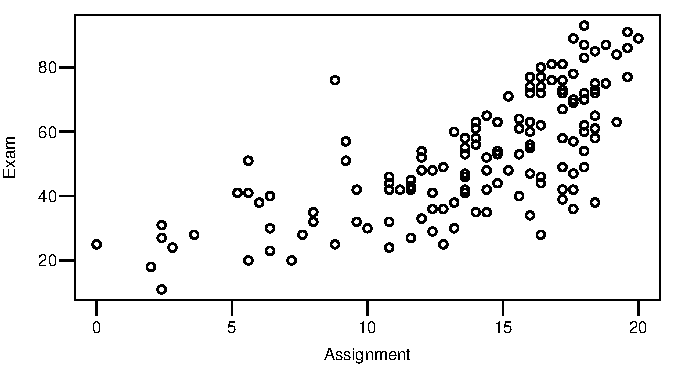
\includegraphics{figure/RC-H04-002}
\end{figure}

Hmmm, not quite a straight line -- could be some curvature. \\
Maybe \rcode{trendscatter} will paint a clearer picture.

\end{frame}


\begin{frame}[fragile]
\frametitle{Exam vs.\ assignment marks\ldots}
\framesubtitle{Scatterplot with trend line}

\begin{knitrout}\scriptsize
\definecolor{shadecolor}{rgb}{0.969, 0.969, 0.969}\color{fgcolor}\begin{kframe}
\begin{alltt}
\hlstd{> }\hlkwd{trendscatter}\hlstd{(Exam} \hlopt{~} \hlstd{Assign,} \hlkwc{data} \hlstd{= Stats20x.df,}\hlkwc{xlab}\hlstd{=}\hlstr{"Assignment"}\hlstd{)}
\end{alltt}
\end{kframe}
\end{knitrout}



\begin{figure}
  \centering
  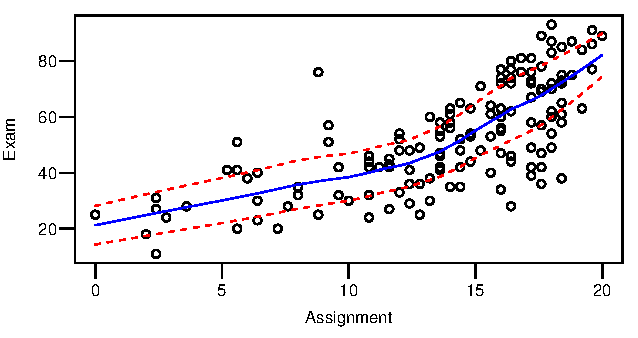
\includegraphics{figure/RC-H04-004}
\end{figure}

Sure looks like some curvature, but, at least the scatter looks fairly constant around this curve.

\end{frame}


\begin{frame}[fragile]
\frametitle{Exam vs.\ assignment marks\ldots}
\framesubtitle{Simple linear model}
Let's fit a simple linear model to these data and see if it works out or not.
\begin{knitrout}\scriptsize
\definecolor{shadecolor}{rgb}{0.969, 0.969, 0.969}\color{fgcolor}\begin{kframe}
\begin{alltt}
\hlstd{> }\hlstd{examassign.fit}\hlkwb{=}\hlkwd{lm}\hlstd{(Exam}\hlopt{~} \hlstd{Assign,}\hlkwc{data} \hlstd{= Stats20x.df)}
\hlstd{> }\hlkwd{plot}\hlstd{(examassign.fit,}\hlkwc{which}\hlstd{=}\hlnum{1}\hlstd{)}
\end{alltt}
\end{kframe}
\end{knitrout}




\begin{figure}
  \centering
  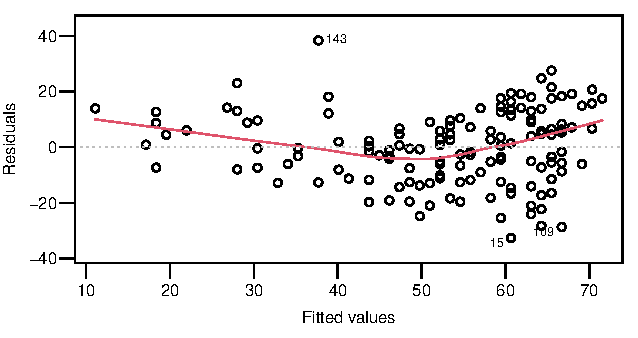
\includegraphics{figure/RC-H04-008}
\end{figure}

Not surprisingly, we still have a curved relationship.
\end{frame}


\begin{frame}[fragile]
\frametitle{Exam vs.\ assignment marks\ldots}
\framesubtitle{Dealing with curvature}
The assumption of identical distribution with expected value of 0 looks to be questionable here.
There tend to be more negative residuals in the middle, but more positive residuals at the extremes of the fitted values.

\bigskip

Potential solution -- add a quadratic (squared term) for \rcode{Assign}.
\end{frame}



%%%%%%%%%%%%%%%%%%%%%%%%%%%%%%%%%%%%%%%%%%%%%%%%%%%%%%%%%%%%%%%%%%%%%%%%%%%%%%%%%%%%%%%%%%%
\BeginSection{Fitting a quadratic model}
%%%%%%%%%%%%%%%%%%%%%%%%%%%%%%%%%%%%%%%%%%%%%%%%%%%%%%%%%%%%%%%%%%%%%%%%%%%%%%%%%%%%%%%%%%%

\begin{frame}[fragile]
\frametitle{The quadratic curve} 
The standard notation for a quadratic curve is\footnote{If you have done a bit of 
calculus, then you might recall that the roots (the values of $x$ that give $y=0$) of a 
quadratic are $\frac{-b \pm \sqrt{b^2-4ac}}{2a}$. }
\[ 
y = a x^2 + b x + c 
\]
Here we will use different notation: 
$\beta_0 \equiv c$, $\beta_1=b$ and $\beta_2=a$ and use the quadratic curve to
describe the expected value of our dependent variable $y$.
That is,
\[ 
\E[Y|x] = \beta_0 + \beta_1 x + \beta_2 x^2 
\]
This is a linear model with explanatory terms $x$ and $x^2$ -- remember, the intercept $\beta_0$ is implicitly included.
\end{frame}


\begin{frame}[ fragile]
\frametitle{The quadratic curve\ldots}
If $\beta_2>0$, then the quadratic has slope that increases with increasing $x$:
\begin{knitrout}\scriptsize
\definecolor{shadecolor}{rgb}{0.969, 0.969, 0.969}\color{fgcolor}
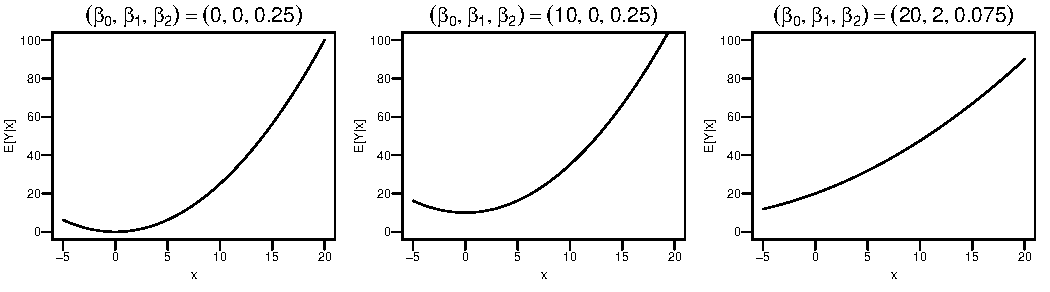
\includegraphics[width=\maxwidth]{figure/RC-H04-009-1} 
\end{knitrout}

If $\beta_2<0$, then the quadratic has slope that decreases with increasing $x$:
\begin{knitrout}\scriptsize
\definecolor{shadecolor}{rgb}{0.969, 0.969, 0.969}\color{fgcolor}
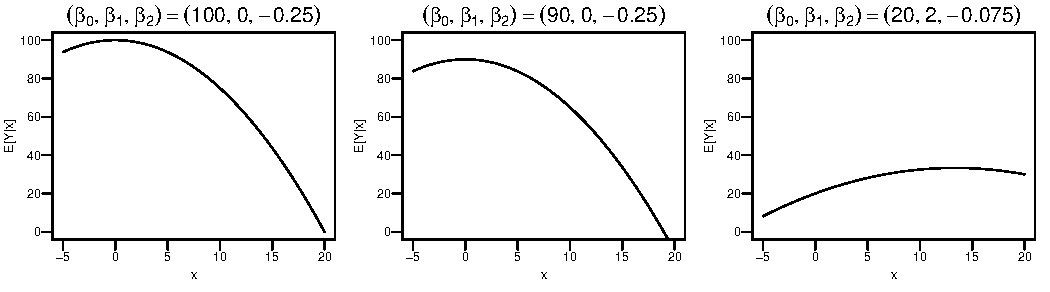
\includegraphics[width=\maxwidth]{figure/RC-H04-010-1} 
\end{knitrout}
\end{frame}


\begin{frame}[ fragile]
\frametitle{How can a quadratic be a linear model?}
\framesubtitle{(Non-examinable)}
Throughout this course, when we use the term ``linear model'' we mean a model that is linear with respect to the $\beta$ coefficients. 
\medskip

This mean that the derivative of the linear model with respect to any $\beta$ coefficient is a constant.
\medskip

The quadratic curve model
\[ 
\E[Y|x] = \beta_0 + \beta_1 x + \beta_2 x^2 
\]
is a quadratic model for $x$.
\medskip

The derivatives of this quadratic with respect to $\beta_0$, $\beta_1$ and $\beta_2$ are 1, $x$ and $x^2$, respectively. These derivatives are all considered ``constants'' because they do not depend on any $\beta$ coefficient. 
\medskip

That is, the quadratic (in $x$) model is linear in $\beta_0$, $\beta_1$ and $\beta_2$.
\end{frame}



\begin{frame}[ fragile]
\frametitle{Exam vs.\ assignment marks\ldots}
\framesubtitle{Adding a squared term}

Add a squared term for \rcode{Assign} via \rcode{I(Assign\string^2)}, like this:\footnote{
\textbf{NOTE:} In the \rcode{lm} formula it is necessary to enclose the \rcode{Assign\string^2} term
inside \rcode{I()} so that \rcode{lm} can make sense of it.}

\begin{knitrout}\scriptsize
\definecolor{shadecolor}{rgb}{0.969, 0.969, 0.969}\color{fgcolor}\begin{kframe}
\begin{alltt}
\hlstd{> }\hlstd{examassign.fit2}\hlkwb{=}\hlkwd{lm}\hlstd{(Exam}\hlopt{~} \hlstd{Assign} \hlopt{+} \hlkwd{I}\hlstd{(Assign}\hlopt{^}\hlnum{2}\hlstd{),} \hlkwc{data} \hlstd{= Stats20x.df)}
\hlstd{> }\hlkwd{plot}\hlstd{(examassign.fit2,}\hlkwc{which}\hlstd{=}\hlnum{1}\hlstd{)}
\end{alltt}
\end{kframe}
\end{knitrout}


\vspace{-3mm}

\begin{figure}
  \centering
  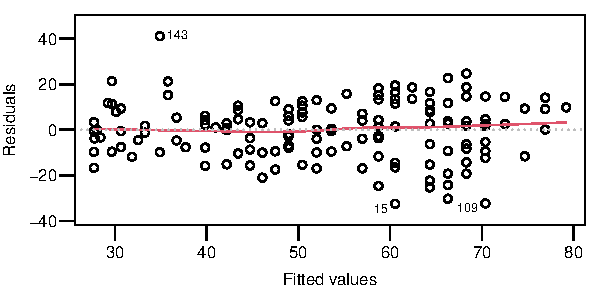
\includegraphics{figure/RC-H04-012}
\end{figure}

\vspace{-3mm}
That is looking much better.
\end{frame}


\begin{frame}[ fragile]
\frametitle{Exam vs.\ assignment marks\ldots}
\framesubtitle{Normality check of the quadratic model}
\begin{knitrout}\scriptsize
\definecolor{shadecolor}{rgb}{0.969, 0.969, 0.969}\color{fgcolor}\begin{kframe}
\begin{alltt}
\hlstd{> }\hlkwd{normcheck}\hlstd{(examassign.fit2)}
\end{alltt}
\end{kframe}
\end{knitrout}



\begin{figure}
  \centering
  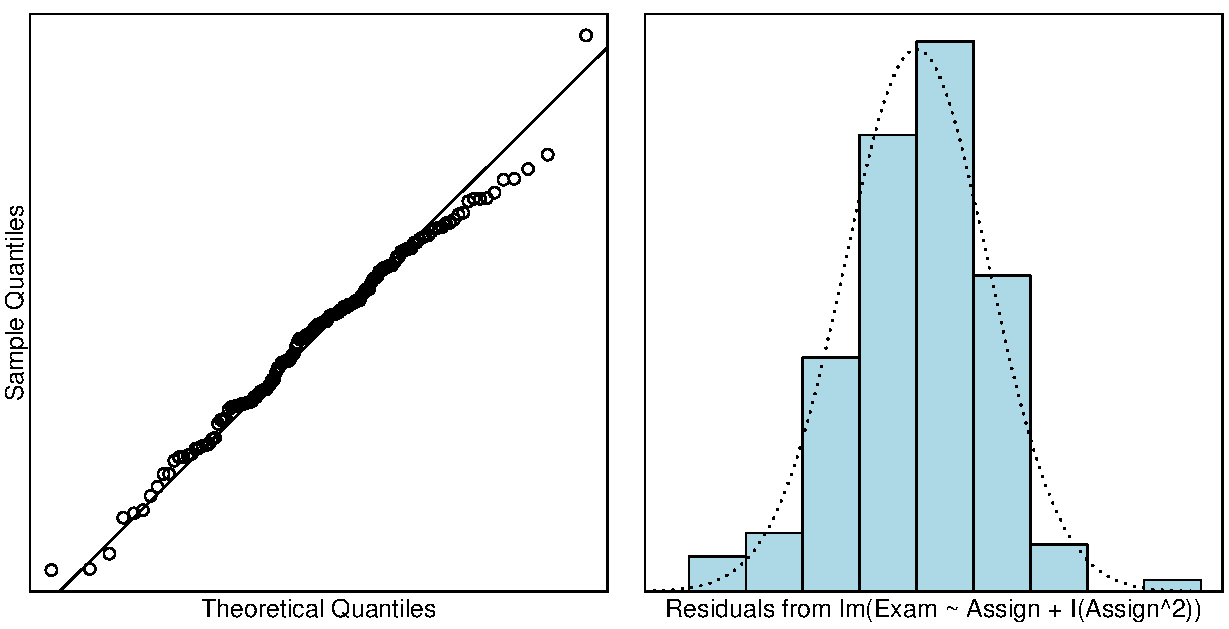
\includegraphics[scale=0.5]{figure/RC-H04-014}
\end{figure}
 
Looking good. There is one potential outlier. Let us check if it is influential.
\end{frame}


\begin{frame}[fragile]
\frametitle{Exam vs.\ assignment marks\ldots}
\framesubtitle{Influence check of the quadratic model}

\begin{knitrout}\scriptsize
\definecolor{shadecolor}{rgb}{0.969, 0.969, 0.969}\color{fgcolor}\begin{kframe}
\begin{alltt}
\hlstd{> }\hlkwd{cooks20x}\hlstd{(examassign.fit2)}
\end{alltt}
\end{kframe}
\end{knitrout}



\begin{figure}
  \centering
  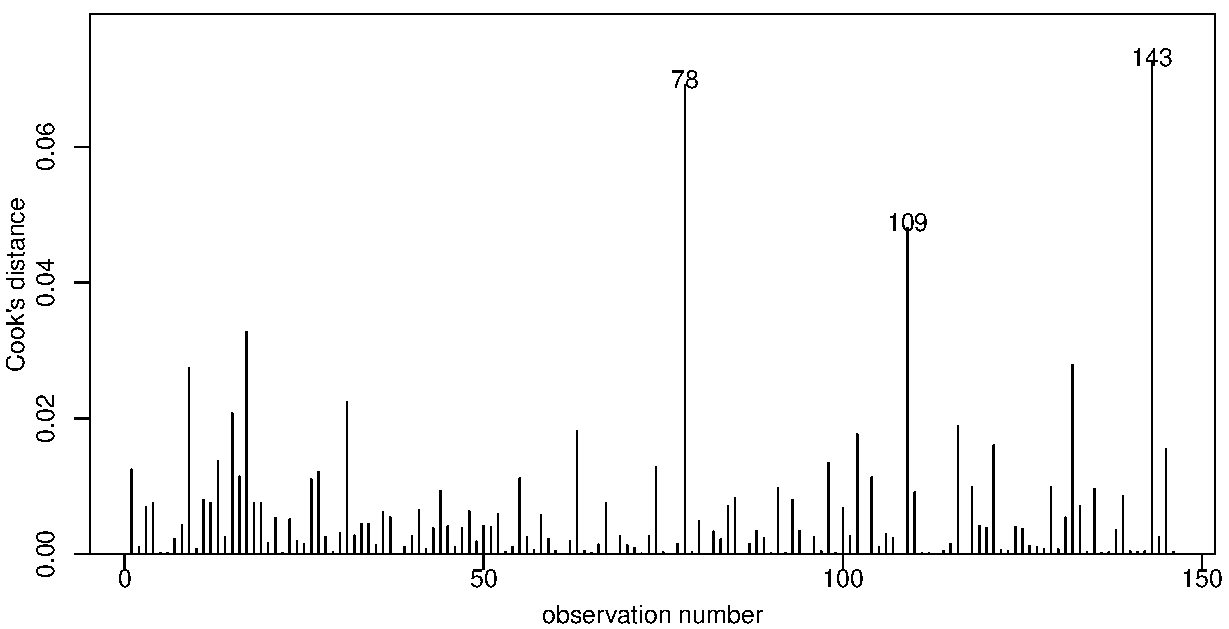
\includegraphics[scale=0.5]{figure/RC-H04-016}
\end{figure}

No high influence points.
\end{frame}


\begin{frame}[fragile]
\frametitle{Exam vs.\ assignment marks\ldots}
\framesubtitle{The fitted models}

We have fitted a quadratic to see if we can add the `curviness' in the relationship between test score and exam mark into our model.
\medskip

Let us compare the two models visually -- model 1 (linear) in {\color{red}red} and  model 2 (quadratic) in {\color{blue}blue}.

\begin{knitrout}\scriptsize
\definecolor{shadecolor}{rgb}{0.969, 0.969, 0.969}\color{fgcolor}\begin{kframe}
\begin{alltt}
\hlstd{> }\hlkwd{plot}\hlstd{(Exam}\hlopt{~} \hlstd{Assign,} \hlkwc{data} \hlstd{= Stats20x.df,} \hlkwc{xlab}\hlstd{=}\hlstr{"Assignment"}\hlstd{)}
\hlstd{> }\hlstd{x}\hlkwb{=}\hlnum{0}\hlopt{:}\hlnum{20} \hlcom{#Assignment values at which to predict exam mark}
\hlstd{> }\hlcom{## Plot model 1}
\hlstd{> }\hlkwd{lines}\hlstd{(x,} \hlkwd{predict}\hlstd{(examassign.fit,}\hlkwd{data.frame}\hlstd{(}\hlkwc{Assign}\hlstd{=x)),} \hlkwc{col}\hlstd{=}\hlstr{"red"}\hlstd{)}
\hlstd{> }\hlcom{## Plot model 2}
\hlstd{> }\hlkwd{lines}\hlstd{(x,} \hlkwd{predict}\hlstd{(examassign.fit2,}\hlkwd{data.frame}\hlstd{(}\hlkwc{Assign}\hlstd{=x)),} \hlkwc{col}\hlstd{=}\hlstr{"blue"}\hlstd{)}
\end{alltt}
\end{kframe}
\end{knitrout}
\end{frame}

\begin{frame}[fragile]
\frametitle{Exam vs.\ assignment marks\ldots}
\framesubtitle{The fitted models\ldots}



\begin{figure}
  \centering
  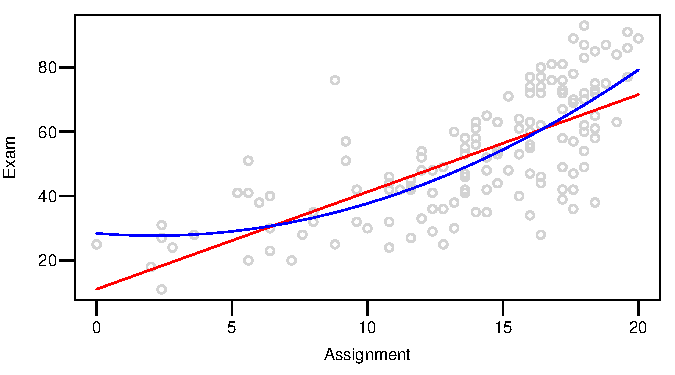
\includegraphics{figure/RC-H04-018}
\end{figure}

\end{frame}

\begin{frame}[fragile]
\frametitle{Exam vs.\ assignment marks\ldots}
\framesubtitle{The fitted quadratic model}

To plot the quadratic over a wider range of \rcode{x} (\rcode{=Assign}) values we can use the following code:

\begin{knitrout}\scriptsize
\definecolor{shadecolor}{rgb}{0.969, 0.969, 0.969}\color{fgcolor}\begin{kframe}
\begin{alltt}
\hlstd{> }\hlstd{x}\hlkwb{=}\hlkwd{seq}\hlstd{(}\hlopt{-}\hlnum{15}\hlstd{,} \hlnum{25}\hlstd{,}\hlkwc{by} \hlstd{=}\hlnum{.10}\hlstd{)} \hlcom{#Sequence of from -15 to 25, in steps of 0.1}
\hlstd{> }
\hlstd{> }\hlstd{y}\hlkwb{=}\hlkwd{predict}\hlstd{(examassign.fit2,}\hlkwc{newdata} \hlstd{=} \hlkwd{data.frame}\hlstd{(}\hlkwc{Assign}\hlstd{=x))}
\hlstd{> }\hlkwd{plot}\hlstd{(y}\hlopt{~}\hlstd{x,} \hlkwc{type}\hlstd{=}\hlstr{"l"}\hlstd{,}\hlkwc{lty}\hlstd{=}\hlnum{2}\hlstd{)}
\hlstd{> }
\hlstd{> }\hlcom{## The bits we want,  0<=x<=20 - N.B. Here & (ampersand) = AND}
\hlstd{> }\hlkwd{lines}\hlstd{(x[x}\hlopt{>=}\hlnum{0}\hlopt{&}\hlstd{x}\hlopt{<=}\hlnum{20}\hlstd{],y[x}\hlopt{>=}\hlnum{0}\hlopt{&}\hlstd{x}\hlopt{<=}\hlnum{20}\hlstd{],}\hlkwc{col}\hlstd{=}\hlstr{"blue"}\hlstd{)}
\hlstd{> }
\hlstd{> }\hlcom{## The range of assign & exam respectively}
\hlstd{> }\hlkwd{abline}\hlstd{(}\hlkwc{v}\hlstd{=}\hlkwd{range}\hlstd{(Stats20x.df}\hlopt{$}\hlstd{Assign),}\hlkwc{lty}\hlstd{=}\hlnum{2}\hlstd{,} \hlkwc{col}\hlstd{=}\hlstr{"grey"}\hlstd{)}
\hlstd{> }\hlkwd{abline}\hlstd{(}\hlkwc{h}\hlstd{=}\hlkwd{c}\hlstd{(}\hlnum{0}\hlstd{,}\hlnum{100}\hlstd{),}\hlkwc{lty}\hlstd{=}\hlnum{2}\hlstd{,} \hlkwc{col}\hlstd{=}\hlstr{"grey"}\hlstd{)}
\end{alltt}
\end{kframe}
\end{knitrout}

\end{frame}

\begin{frame}[fragile]
\frametitle{Exam vs.\ assignment marks\ldots}
\framesubtitle{The fitted quadratic model\ldots}


\begin{figure}
  \centering
  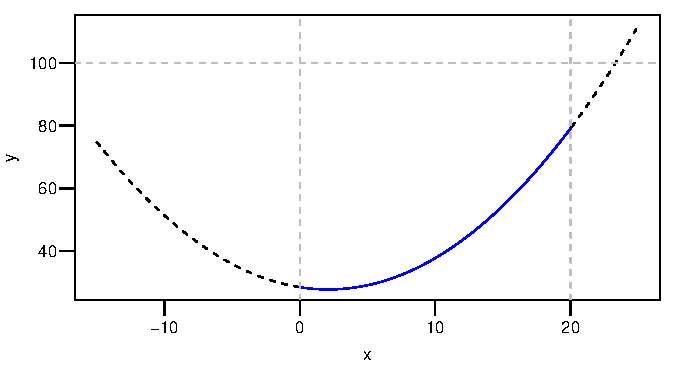
\includegraphics{figure/RC-H04-020}
\end{figure}

\end{frame}


\begin{frame}[ fragile]
\frametitle{Exam vs.\ assignment marks\ldots}
\framesubtitle{Comparison of straight line and quadratic models}

\begin{small}
\begin{knitrout}\scriptsize
\definecolor{shadecolor}{rgb}{0.969, 0.969, 0.969}\color{fgcolor}\begin{kframe}
\begin{alltt}
\hlstd{> }\hlkwd{summary}\hlstd{(examassign.fit)}   \hlcom{## Straight line model}
\end{alltt}
\end{kframe}
\end{knitrout}

\begin{knitrout}\scriptsize
\definecolor{shadecolor}{rgb}{0.969, 0.969, 0.969}\color{fgcolor}\begin{kframe}
\begin{verbatim}
Coefficients:
            Estimate Std. Error t value Pr(>|t|)    
(Intercept)  11.0874     3.5954   3.084  0.00245 ** 
Assign        3.0222     0.2478  12.195  < 2e-16 ***
---
Residual standard error: 13.15 on 144 degrees of freedom
Multiple R-squared:  0.508,	Adjusted R-squared:  0.5046 
F-statistic: 148.7 on 1 and 144 DF,  p-value: < 2.2e-16
\end{verbatim}
\end{kframe}
\end{knitrout}

\begin{knitrout}\scriptsize
\definecolor{shadecolor}{rgb}{0.969, 0.969, 0.969}\color{fgcolor}\begin{kframe}
\begin{alltt}
\hlstd{> }\hlkwd{summary}\hlstd{(examassign.fit2)}  \hlcom{## Model with quadratic term}
\end{alltt}
\end{kframe}
\end{knitrout}

\begin{knitrout}\scriptsize
\definecolor{shadecolor}{rgb}{0.969, 0.969, 0.969}\color{fgcolor}\begin{kframe}
\begin{verbatim}
Coefficients:
            Estimate Std. Error t value Pr(>|t|)    
(Intercept) 28.41396    5.99081   4.743 5.05e-06 ***
Assign      -0.68172    1.07242  -0.636 0.525999    
I(Assign^2)  0.16102    0.04545   3.542 0.000536 ***
---
Residual standard error: 12.65 on 143 degrees of freedom
Multiple R-squared:  0.5477,	Adjusted R-squared:  0.5414 
F-statistic: 86.59 on 2 and 143 DF,  p-value: < 2.2e-16
\end{verbatim}
\end{kframe}
\end{knitrout}
\end{small}
\end{frame}

\begin{frame}[ fragile]
\frametitle{Exam vs.\ assignment marks\ldots}
\framesubtitle{Comparison of straight line and quadratic models\ldots}

The small \pval{} $(=0.000536$) for testing $H_0: \beta_2=0$ tells us that that the quadratic term is statistically significant. 
Our model went from:

\medskip
$ Exam_i =\beta_0+\beta_1\times Assign_i +\varepsilon_i$  ~where~ $\varepsilon_i \iid N(0,\sigma^2)$ to

\medskip 

$ Exam_i =\beta_0+\beta_1\times Assign_i +\beta_2\times Assign_i^2 + \varepsilon_i$ ~where~ $\varepsilon_i \iid N(0,\sigma^2)$.

\medskip 
Note that the coefficient $\beta_2>0$ associated with the \rcode{I(Assign)\string^2} term
results in an improvement in expected exam score that `accelerates' as \rcode{Assign} increases.

\medskip 
We could consider removing the non-significant `straight line' \rcode{Assign} term. 
\textbf{What would you do?}

\medskip 

We have done a better job of modelling this data by adding this extra term, and the $R^2$ explained another 4\% of the total variation.

\medskip 
\textbf{MORAL:} If it looks like a curve  then  fit a curve  --  \underline{provided} the scatter about the curve is constant (\textbf{EOV}).

\end{frame}



%%%%%%%%%%%%%%%%%%%%%%%%%%%%%%%%%%%%%%%%%%%%%%%%%%%%%%%%%%%%%%%%%%%%%%%%%%%%%%%%%%%%%%%%%%%
\BeginSection{Relevant \rcode{R}-code}
%%%%%%%%%%%%%%%%%%%%%%%%%%%%%%%%%%%%%%%%%%%%%%%%%%%%%%%%%%%%%%%%%%%%%%%%%%%%%%%%%%%%%%%%%%%



\begin{frame}[fragile]
\frametitle{Most of the \rcode{R}-code you need for this chapter}

If you suspect the relationship between your $x$ and $y$ variables follows a curve rather than a straight line (as revealed in the plot of residuals vs fitted values), and the scatter remains constant around this curve, then fit a quadratic:
\bigskip

\begin{knitrout}\scriptsize
\definecolor{shadecolor}{rgb}{0.969, 0.969, 0.969}\color{fgcolor}\begin{kframe}
\begin{alltt}
\hlstd{> }\hlstd{examassign.fit2}\hlkwb{=}\hlkwd{lm}\hlstd{(Exam}\hlopt{~} \hlstd{Assign} \hlopt{+} \hlkwd{I}\hlstd{(Assign}\hlopt{^}\hlnum{2}\hlstd{),} \hlkwc{data} \hlstd{= Stats20x.df)}
\hlstd{> }\hlcom{#Check the residual plot again - hopefully the curvature is gone.}
\hlstd{> }\hlkwd{plot}\hlstd{(examassign.fit2,}\hlkwc{which}\hlstd{=}\hlnum{1}\hlstd{)}
\end{alltt}
\end{kframe}
\end{knitrout}
\bigskip

{\bf NOTE:} If the null hypothesis $H_0: \beta_2=0$ is {\bf not} rejected (i.e, \pval{}$>0.05$), then our preferred model would be the simple linear regression model.
\end{frame}




\end{document}
